\chapter{Project Management}
\label{ch:projectmanagement}

\section{Project Method}
\label{section:projectmethod}
We will be using the SCRUM process for organising our work.
This means splitting the work packages into stories and scheduling for completion in sprints.
Sprints shall last two weeks. At the end of every sprint the progress is reviewed with the advisors and the next sprint is planned.

\section{Project Timeline}
\label{section:projecttimeline}
Since we know in advance the timeframes within we must complete our work, we created the following project timeline.

\begin{landscape}
\topskip0pt
\vspace*{\fill}
	\begin{figure}[H]
	\begin{center}
		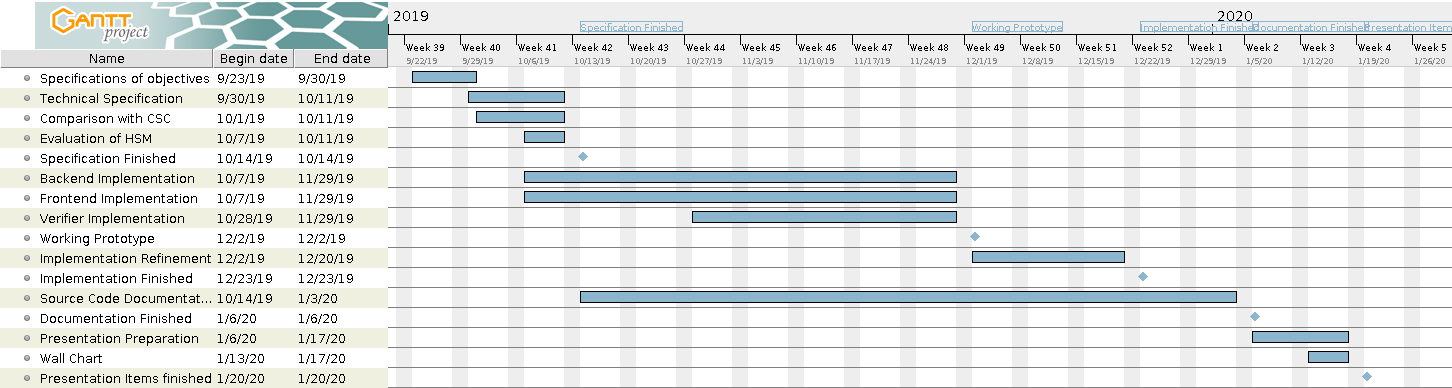
\includegraphics[scale=0.5]{images/Projectplan.png}
		\caption{Project timeline}
		\label{fig:projecttimeline}
	\end{center}
	\end{figure}
\vspace*{\fill}
\end{landscape}

\section{Work Packages}
\label{section:workpackages}

\subsection{Specification of Objectives}
The objectives of our thesis will be specified.
This included functional and non-functional requirements.

\subsection{Technical Specification}
The requirements defined in the objectives will be mapped to concrete technology choices.
Also the choice of languages and frameworks will be explained.

\subsection{Comparison with CSC Implementation}
We will compare our Specification with the Remote Signing Standard specified by the \gls{CSC}.

\subsection{Evaluation of Yubikey HSM}
We will evaluate how we can use the Yubikey HSM for our Signature Service.

\subsection{Backend Implementation}
The backend consisting of the Signing Service and the OIDC Coupling with the IDP will be implemented.

\subsection{Frontend Implementation}
The frontend consisting of the Hashing and UI will be implemented.

\subsection{Standalone Verifier Implementation}
The application for the offline verification of the signature will be implemented.

\subsection{Implementation Refinement}
After the working prototype, eventual bugs will be fixed and optional goals will be implemented.

\subsection{Source Code Documentation}
We will document the source code.

\subsection{Presentation}
We will create the slides and prepare the presentation.

\subsection{Wall Chart and Article}
We will create a wall chart and short article describing our work.

\subsection{Video}
We will create a short video introducing our problem.